\documentclass[border=6pt,12pt]{standalone}
\usepackage{times}
\usepackage{inconsolata}
\usepackage[T1]{fontenc}
\usepackage{amsmath,amssymb,booktabs,xcolor}
\usepackage{tikz}
\usetikzlibrary{arrows.meta, positioning, shadows, calc}
\begin{document}
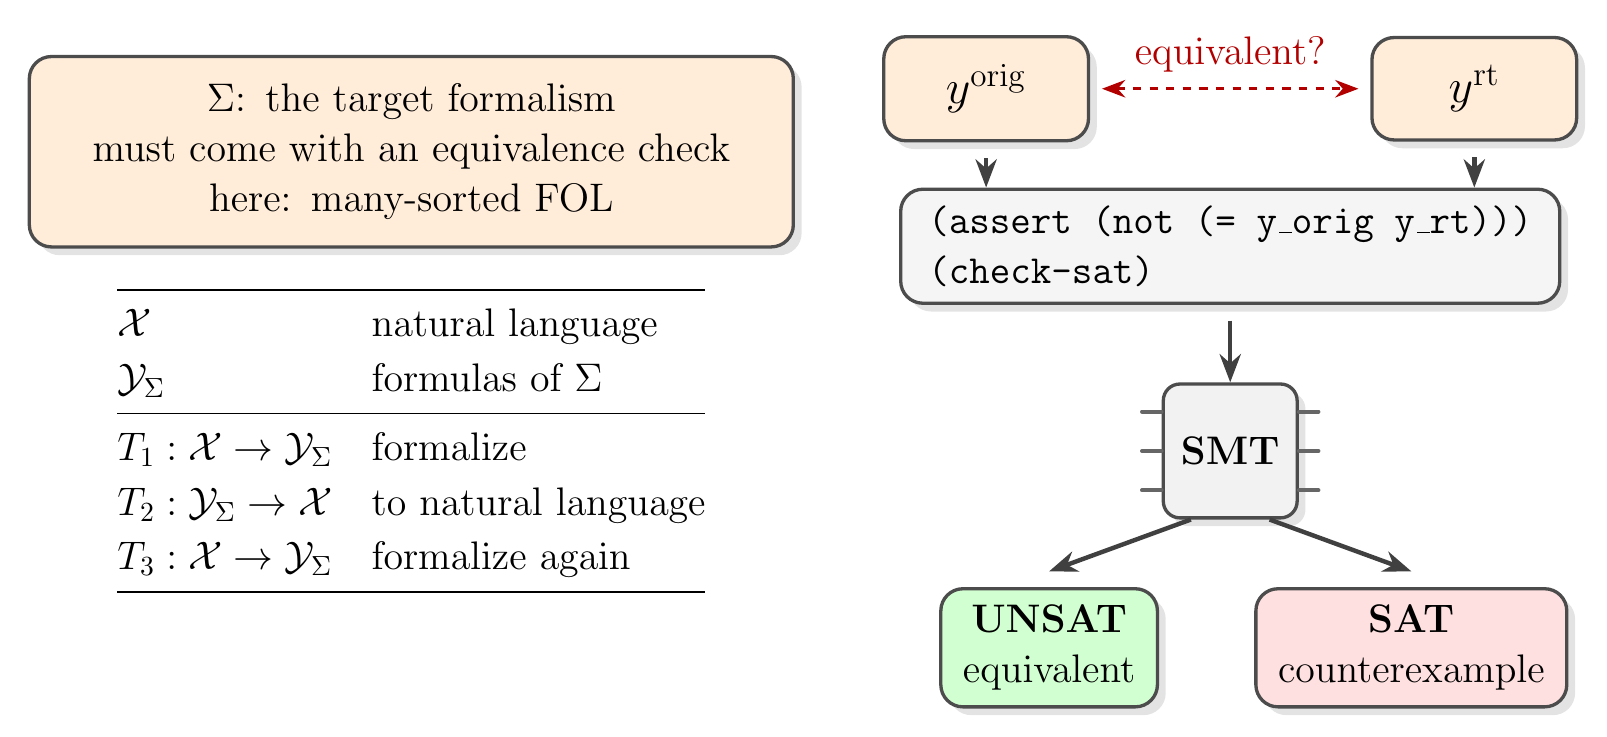
\begin{tikzpicture}[>=Stealth, font=\Large,
  card/.style={draw=black!70, line width=1.2pt, rounded corners=8pt, inner sep=10pt,
               drop shadow={opacity=0.22, shadow xshift=3pt, shadow yshift=-3pt}},
  fmcard/.style={card, fill=orange!15, align=center, font=\LARGE, minimum width=2.6cm, minimum height=1.1cm},
  codecard/.style={card, fill=black!4, align=left, font=\Large\ttfamily, inner ysep=6pt},
  verdict/.style={card, align=center, inner xsep=8pt, inner ysep=6pt, minimum height=1.0cm},
  chip/.style={draw=black!70, line width=1.2pt, rounded corners=6pt, fill=black!5,
               minimum size=1.7cm, font=\Large\bfseries, inner sep=4pt,
               drop shadow={opacity=0.22, shadow xshift=3pt, shadow yshift=-3pt}},
  pin/.style={draw=black!60, line width=1.4pt, line cap=round},
  arr/.style={->, line width=1.6pt, black!75},
]
% ---------- right half: the check as a diagram ----------
\node[fmcard] (yo) at (-3.1, 3.1) {$y^{\mathrm{orig}}$};
\node[fmcard] (yr) at ( 3.1, 3.1) {$y^{\mathrm{rt}}$};
\draw[{Stealth}-{Stealth}, dashed, line width=1.2pt, red!70!black]
  ([xshift=0.15cm]yo.east) -- node[above=2pt, text=red!70!black] {equivalent?} ([xshift=-0.15cm]yr.west);
\node[codecard] (q) at (0, 1.1) {(assert (not (= y\_orig y\_rt)))\\(check-sat)};
\draw[arr] ([yshift=-0.2cm]yo.south) -- (yo.south |- q.north);
\draw[arr] ([yshift=-0.2cm]yr.south) -- (yr.south |- q.north);
\node[chip] (smt) at (0, -1.5) {SMT};
\foreach \y in {-0.5,0,0.5} {
  \draw[pin] ([yshift=\y cm]smt.west) -- ++(-0.25,0);
  \draw[pin] ([yshift=\y cm]smt.east) -- ++(0.25,0);
}
\draw[arr] ([yshift=-0.2cm]q.south) -- (smt.north);
\node[verdict, fill=green!18] (ok)  at (-2.3, -4.0) {\textbf{UNSAT}\\equivalent};
\node[verdict, fill=red!12]   (bad) at ( 2.3, -4.0) {\textbf{SAT}\\counterexample};
\draw[arr] ([xshift=-0.5cm]smt.south) -- ([yshift=0.2cm]ok.north);
\draw[arr] ([xshift= 0.5cm]smt.south) -- ([yshift=0.2cm]bad.north);
% ---------- left half: the formal objects ----------
\node[card, fill=orange!15, align=center, text width=9.0cm] (sig) at (-10.4, 2.3)
  {$\Sigma$: the target formalism\\ must come with an equivalence check\\ here: many-sorted FOL};
\node[anchor=north, inner sep=0pt] (tab) at ([yshift=-0.5cm]sig.south) {%
\renewcommand{\arraystretch}{1.1}%
\begin{tabular}{@{}l@{\quad}l@{}}
\toprule
$\mathcal{X}$ & natural language \\
$\mathcal{Y}_{\Sigma}$ & formulas of $\Sigma$ \\
\midrule
$T_1 : \mathcal{X} \rightarrow \mathcal{Y}_{\Sigma}$ & formalize \\
$T_2 : \mathcal{Y}_{\Sigma} \rightarrow \mathcal{X}$ & to natural language \\
$T_3 : \mathcal{X} \rightarrow \mathcal{Y}_{\Sigma}$ & formalize again \\
\bottomrule
\end{tabular}};
\end{tikzpicture}
\end{document}
